\begin{figure*}[t]
\centering
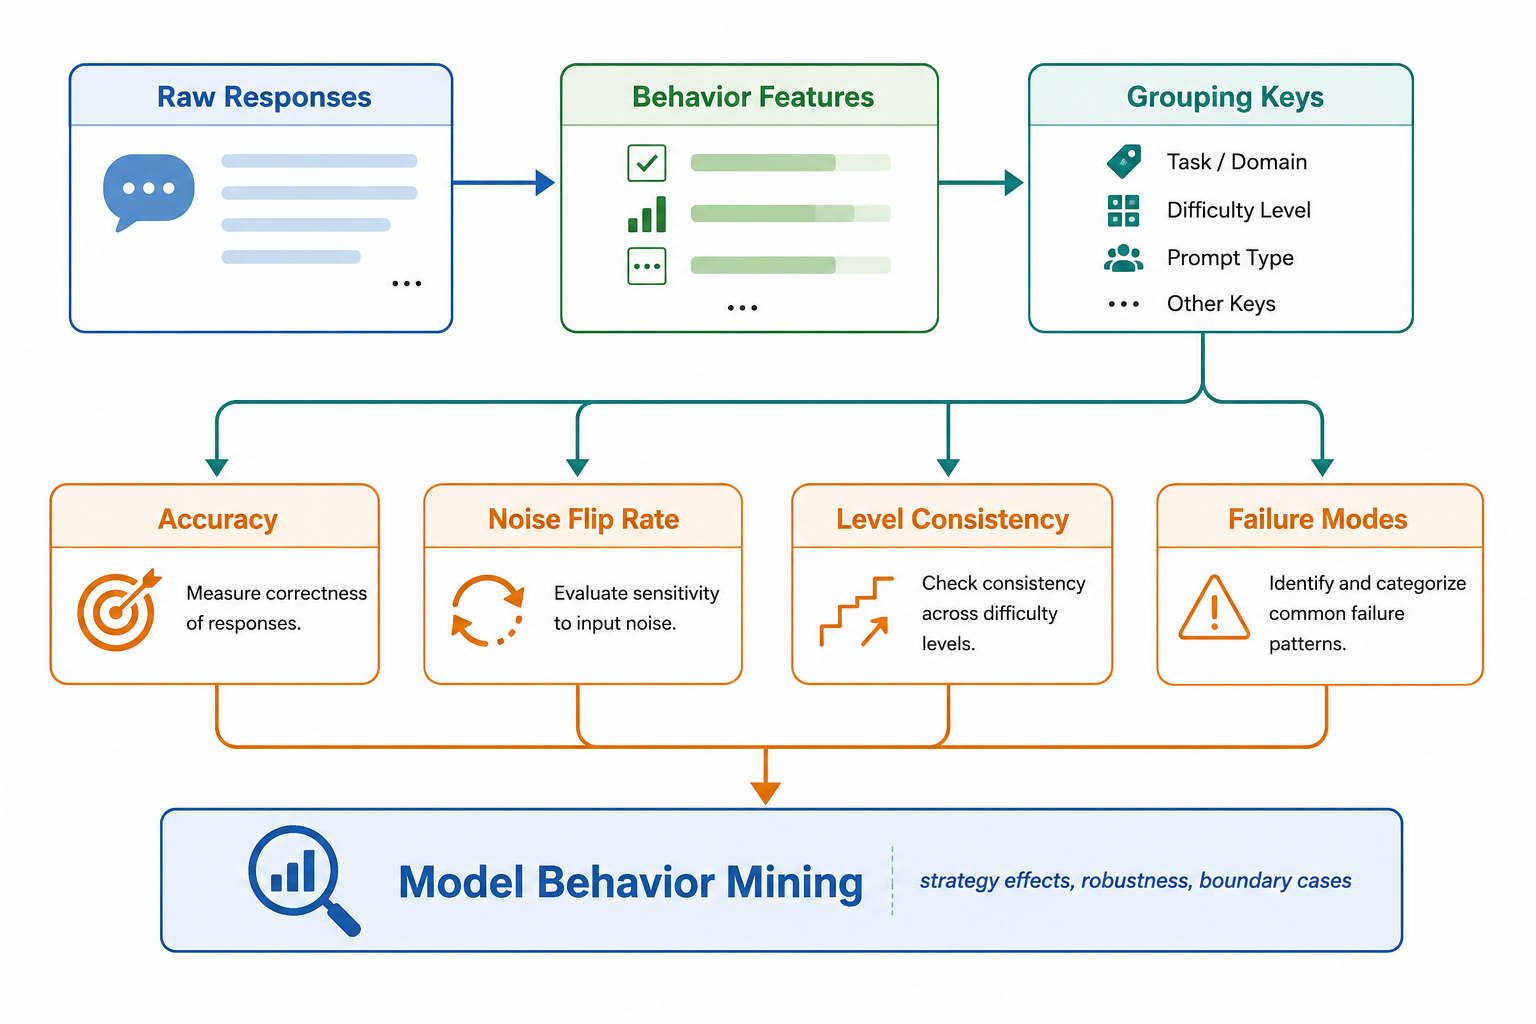
\includegraphics[width=0.74\textwidth,height=0.25\textheight,keepaspectratio]{figures/behavior.png}
\caption{行为数据挖掘框架。原始回复先被解析为结构化特征，再按策略、层级、扰动和模型分组，最终从准确性、噪声翻转、层级一致性和失败模式四个角度解释模型空间推理行为。}
\label{fig:behavior-mining-framework}
\end{figure*}
